\begin{figure*}[t]
    \centering

    \begin{subfigure}[b]{.45\textwidth}
        \centering
        \resizebox{\linewidth}{!}{\includegraphics{figure/plot/reference/fig4-pointer-chasing-heatmap.pdf}}
        \caption{\label{fig:4:ref:ptr-chasing-heatmap}[Ref]}
    \end{subfigure}
    \hfill
    \begin{subfigure}[b]{.45\textwidth}
        \centering
        \resizebox{\linewidth}{!}{\includegraphics{example-image-duck}}
        % \resizebox{\linewidth}{!}{\includegraphics{figure/plot/reproduce/fig4-pointer-chasing-heatmap.pdf}}
        \caption{\label{fig:4:rep:ptr-chasing-heatmap}[Rep]}
    \end{subfigure}

    \caption{Pointer chasing microbenchmark results. The heatmap shows the pointer chasing latency under varying striding sizes and number of blocks. When we have 16 blocks or less, the latency does not increase for any stride size, indicating that we have at least 16 block available, i.e., associativity of 16. }
    \label{fig:4:ptr-chasing-heatmap}
\end{figure*}
